\chapter{Deep learning}
\section{Success stories}
We start this section introducing the two fields that have been spearheading the Deep Learning revolution: computer vision and speech recognition.
The first consists in identifying objects in digital images; while the second is being able to transcribe and process audio.

It is striking that both cases correspond to tasks that humans are very good at.
Indeed, neural networks are very good at \emph{perceptual learning}

\section{The basic blocks}
A deep learning model is composed by a series of layers, or simple transformations (usually linear), plus a point-wise non-linearity.


\subsection{Fully connected layers}
Also known as ``dense" layers, they are the simplest building block of deep learning: a simple matrix multiplication, as described in the Section~\ref{sec:mlp}.
To make them more general, they can include a \emph{bias} term, that is added after the multiplication.

\begin{equation*}
\vec{o} = W \cdot \vec{i} + \vec{b}
\end{equation*}

Every element of the output is a function of every input, so this layer destroys the structure of the data.
On the other hand, since the intermediate layers can be arbitrarily large, it can have a lot of parameters, ie, it can be very expressive.
It is often used as the last layer of the model.

\subsection{Convolutions}
Convolutions capture spatial relationships in the data.

\subsection{Recurrent}
A recurrent layer tries to capture temporal dependencies on arbitrary time steps, such as those of natural language, or repeating motifs in proteins.
They work by taking two inputs: the vector at the current position, and the hidden state of the previous cell.
A simple cell:

\subsection{Non-linearities}
The workhorse of deep learning layers are linear transformations.
The composition of linear transformations is also linear, so in order to rip the benefits of multiple layers we need non-linearities.
For the most part, they are point-wise functions that act on the output of a layer.
Historically, the first non-linearity used was the sigmoid:

\begin{equation*}
f(x) = \frac{1}{1 + e^{- x}}
\end{equation*}

It has the advantage of clipping the range of values between 0 and 1, which makes the network stable with respect to large intermediate values. (Figure~\ref{subfig:sigmoid})
An improvement was the hyperbolic tangent:

\begin{equation*}
f(x) = \tanh(x) = \frac{e^x - e^{-x}}{e^x + e^{-x}},
\end{equation*}
with a similar shape to the sigmoid, but now outputting values between -1 and 1. (Figure~\ref{subfig:tanh})
Being anti-symmetric, it can achieve a stable distribution of outputs with normally weights in the intermediate layers.

\begin{figure}[tb]
	\subcaptionbox{Sigmoid\label{subfig:sigmoid}}{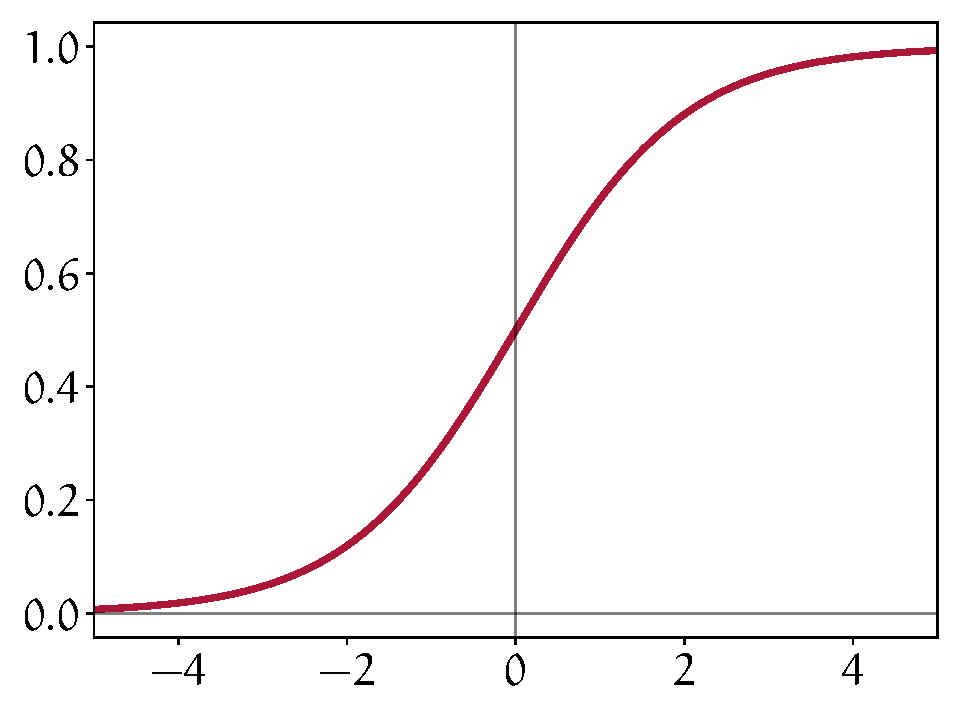
\includegraphics[width=0.45\textwidth]{machine_learning/figures/sigmoid}}
	\hfill
	\subcaptionbox{Tanh\label{subfig:tanh}}{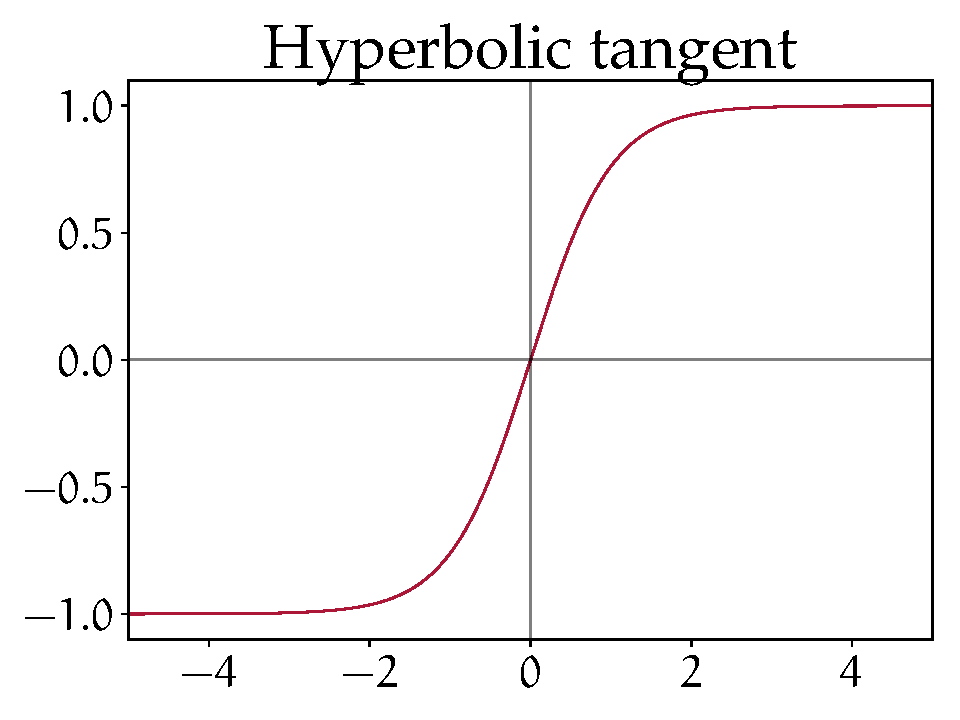
\includegraphics[width=0.45\textwidth]{machine_learning/figures/tanh}}
	\caption{Saturating non-linarities}\label{fig:non_linear}
\end{figure}

Both functions saturate on extreme values, \marginpar{Gradient saturation}
so their derivative approaches zero, which on one hand is useful to control the stability of the outputs, but on the other is a problem for the propagation of gradients.
The alternative is using non-saturating functions, that allow the gradients to flow for a wider range of values.

The simplest is the Rectified Linear Unit, or ReLU, plotted in the Figure~\ref{subfig:relu}:
\begin{equation*}
f(x) =  \begin{cases}
x &  if x \geq 0 \\
0 & otherwise
\end{cases}
\end{equation*}

But in this thesis I have mostly used the Exponential Linear Unit, or ELU, shown in the Figure~\ref{subfig:elu}:
\begin{equation*}
f(x) =  \begin{cases}
x &  if x \geq 0 \\
\frac{1}{1 + e^{-x}} & otherwise
\end{cases}
\end{equation*}

The choice of this non-linearity usually incurs in a slightly larger computational time for training, but a moderate improvement in performance as well.

\begin{figure}[tb]
	\subcaptionbox{ReLU\label{subfig:relu}}{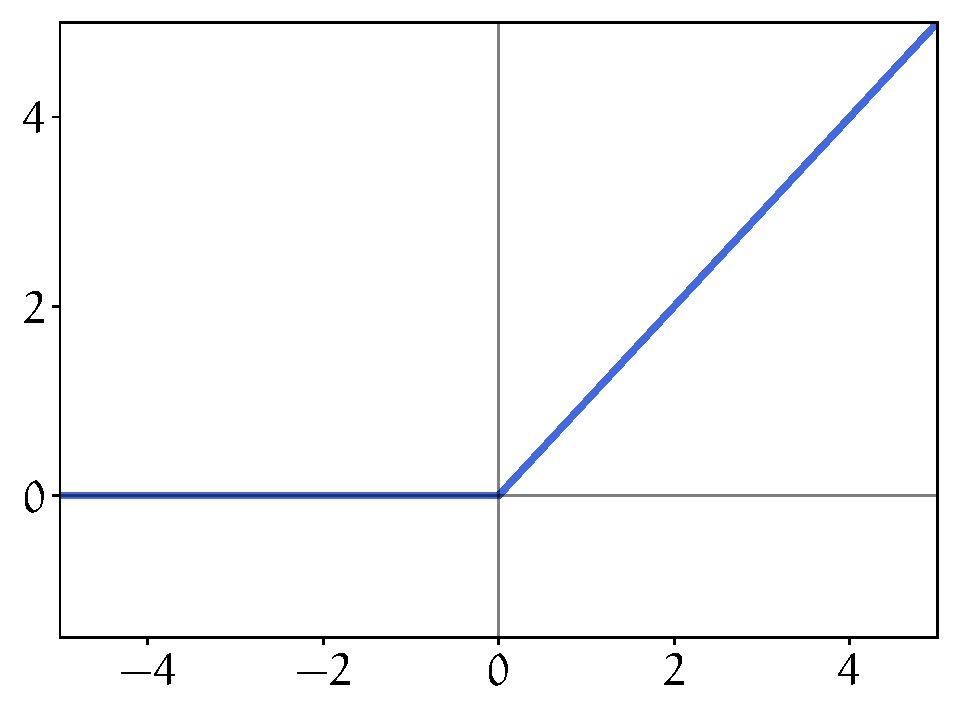
\includegraphics[width=0.45\textwidth]{machine_learning/figures/relu}}
	\hfill
	\subcaptionbox{ELU\label{subfig:elu}}{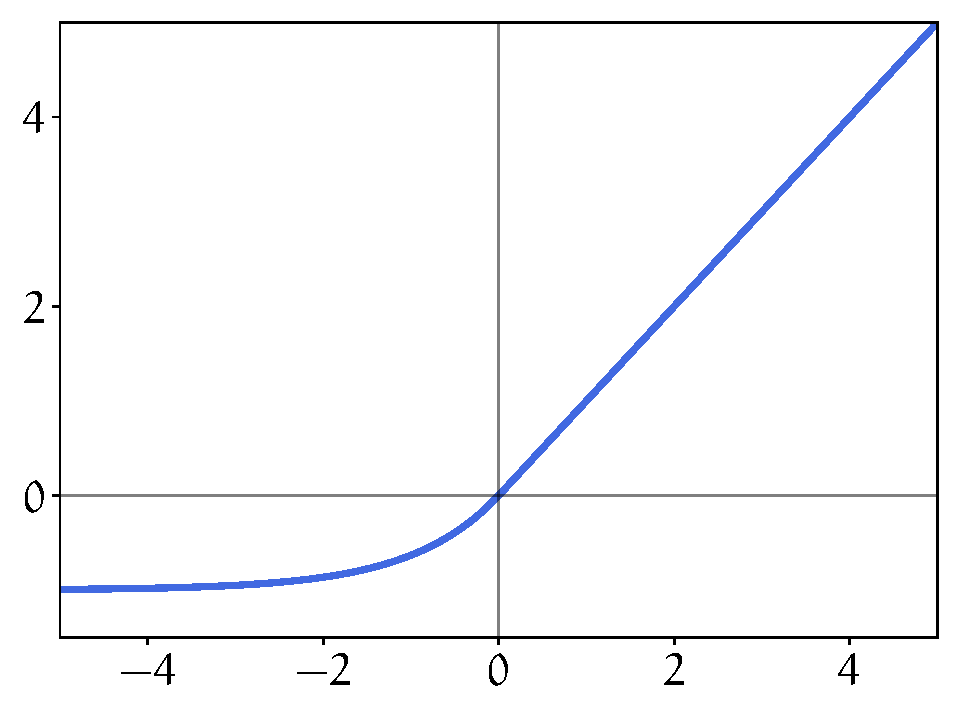
\includegraphics[width=0.45\textwidth]{machine_learning/figures/elu}}
	\caption{Non-saturating non-linarities}\label{fig:non_linear}
\end{figure}

The last layer is an exception.\marginpar{Output}
The function applied depends on the properties of the target.
\begin{itemize}
\item If the output is a binary classification, or multiple mutually compatible classes, use a sigmoid, as described in the Section~\ref{sec:logistic_regression} on logistic regression.
\item If the output are a series of mutually exclusive classes, use a softmax, as explained in the Section~\ref{sec:mlp} on multi layered perceptrons.
\item If the output is a regression, use a linear layer to minimise the squeezing of the outputs.
This is valid even if the output is bounded between 0 and 1, when the values at the extrema are likely to appear, because the network would need to learn very high values for the logits.
\item If the outputs are sines and cosines of angles, use the hyperbolic tangent.
\end{itemize}

\section[Gradient descent]{Training procedure: gradient descent}\label{sec:grad_descent}
A deep learning network can have millions of parameters, but how do we find the optimal values?

In the first place, we need to define a loss function, or a measurement of how wrong our predictions are on known data.
For example, the mean squared error for $N$ data points  $x_i$ with labels $y_i$ and predictions $o_i$ is:

\begin{equation*}
L_{MSE} = \sum_i^N \left(y_i - o_i\right)^2
\end{equation*}
and the cross entropy loss:
\begin{equation*}
L_{H} = \sum_i^N y_i \cdot \log\left(o_i\right) 
\end{equation*}

We initialise the network with random numbers, and measure how wrong we are.
Then, we compute the gradients of the loss with respect to each of the parameters $w_j$ of the network:
\begin{equation*}
g_j = \frac{1}{N}\sum_i^N\frac{\partial L\left(o_i, y_i \right)}{\partial w_j}
\end{equation*}

The gradients tell us in which direction we have to ``nudge" the network to improve its performance for the next iteration:

\begin{equation*}
\left. w_j\right|_{it=k+1} = \left. w_j\right|_{it=k} + \eta \cdot \left. g_j\right|_{it=k},
\end{equation*}
where $\eta$ is the step size, a small number that reflects our believe of the size of the region where the gradients still point in the same direction.

\subsection{Back-propagation}
In order to train, we need to compute the gradients of the loss with respect to all the parameters of the network.
This can be done automatically using the back-propagation algorithm, or \emph{backprop}, the machine version of the chain rule.

\todo[inline]{backprop}

\subsection{Stochastic gradient descent}
\subsection{Optimisers}

\section{Conjunctive tissue: tensors and gradients}

\section{Taming the complexity: regularisation}
Neural networks can have millions of parameters, so they are susceptible to over-fitting.
In order to converge to generalisable models, we can apply a variety of regularisation techniques.
Most of them act as a barrier that hinders the training, that only enough data can overcome.


Here are some:


To prevent any single activation from \marginpar{Weight decay}

$L^2$ regularisation can be interpreted as a Gaussian prior over the weights centred around $0$.

The most popular technique \marginpar{Dropout} 
specifically developed for deep learning is Dropout, \citep{dropout}. 
During training, a random fraction $0 < \rho < 1$ of intermediate inputs is set to $0$ (\emph{dropped out}), while the rest of values are scaled by a factor of $\frac{1}{1-\rho}$ to compensate.

Since the network cannot trust any particular neuron activation to be present, it must distribute the information across different parts.
The architecture is effectively different for every batch, so we are training an ensemble of models, most of which have not seen any data, but are heavily regularised to the average.

\marginpar{Batch Normalisation}

\marginpar{Architectural}

\marginpar{Differential privacy}
Special mention



\section{The quest for depth}
%relu
%batchnorm
%residual

\section{Deep transfer learning}
a


